\chapter{Reorganization of network architecture and its relationship to cognition}

\epigraph{Development...}{Stanislas Dahaene}

\section{Motivation}

To get more at this idea of 

In Study 1, we saw that the degree of modularity of an individual's connectome at rest was positively associated with reading skill. The exception to this was in the cingulo-operculuar and auditory networks, which had a negative correlation; that is, lower segregation of these areas was associated with better reading. In Study 2, we found that tasks, and especially reading comprehension, induced a more integrated network architecture as information was shared across RSNs. However, the relationship between reading skill and modularity persisted, even as connectomes were estimated during separate conditions. Thus, it appears to be the case that better readers have a common and tightly connected network ``backbone'' that is persistent throughout task reconfiguration.

Given that reading is a skill that we know requires a very high degree of cross-RSN interaction, we might expect this to be true in a variety of other domains as well. In fact, we might expect that there would be a high degree of consistency between a number of different tasks: listening and reading, but also attention tasks. 





\section{Methods}

\subsection{Participants}

Participants were drawn from the same cohort of subjects included in Studies 1 and 2, and identical inclusion criteria for both demographic and scan motion were applied. However, additional measures related to the performance of the task were levied as described below. A total of 42 unique subjects and 162 scan sessions were included in the analysis. The demographics for these subjects are described in Table \ref{table:ch3-participants}.

\begin{table}[t]
	\renewcommand{\tabcolsep}{0.09cm}
	\centering
	\begin{tabular}{lc}
\toprule
Measure &               Value \\
\midrule
Subjects                        &              42 \\
Mean age                        &    10.51 (0.33) \\
Sex                             &      21 M, 23 F \\
WASI Full-Scale IQ, Vocabulary  &    52.91 (9.38) \\
Test of Word Reading Efficiency &  104.66 (18.07) \\
\bottomrule
\end{tabular}
	\caption[Participant demographics for Study 3.]{Participant demographics for Study 3.}
	\label{table:ch4-participants}
\end{table}

\subsection{Functional MRI acquisition and processing}

The task design for this study is described in detail in Chapter 3. Briefly, subjects were presented up to four separate runs of a language comprehension task. The task included two passage blocks (``Reading'' or ``Listening''), two sensory baseline blocks (``Attention'') and a trailing resting-state block ("Rest"). The four scan runs were crossed on two conditions: the modality of presentation (auditory or visual) and the genre of the passage (narrative or expository). 

A scan session was excluded based on the following parameters: the number of high-motion volumes exceeding 20 percent, mean frame-wise displacement greater than 0.4, or poor task performance ($D` < 2$). To control for the effects of genre, we matched all scans that met inclusion criteria with their opposing-modality counterpart, so that each subject had either 2 scans (same genre, listening and reading) or 4 scans (both genres, listening and reading). In total, 42 children (162 scans) met inclusion criteria.

Functional MRI acquisition and preprocessing procedures were equivalent to those described for Study 2. See the Methods section of Chapter 3 for a detailed description of these processes and their parameters.

\subsection{Activation analyses}

Our analysis was broken into two parts: first, comparing the similarities and differences in network organization for listening and reading, then across all available tasks. 

For the modality comparisons, we used a fixed-effects subject-level model to estimate the shared activation for ``Listening and Reading'' and their differences ``Listening vs. Reading''. We then used FSL's \textit{randomise} utility to estimate the main effects of modality across all subjects in our sample (5000 permutations, threshold-free cluster enhancement, $p < 0.05$).

We also investigated these effects in ``connectome space'' by extracting the values at each of the 264 nodes used for connectivity analysis. 


\subsection{Network similarity estimation}

There are two methods for estimating network similarity. In the first case, modularity is an estimate:

A direct comparison, without reference to a prior ``parcellation'' is possible using the network \textit{intersection}. In this case, the number of connections shared between two connectivity arrays is a stable estimate of similarity, becuase


\begin{figure}[t]
	\centering
	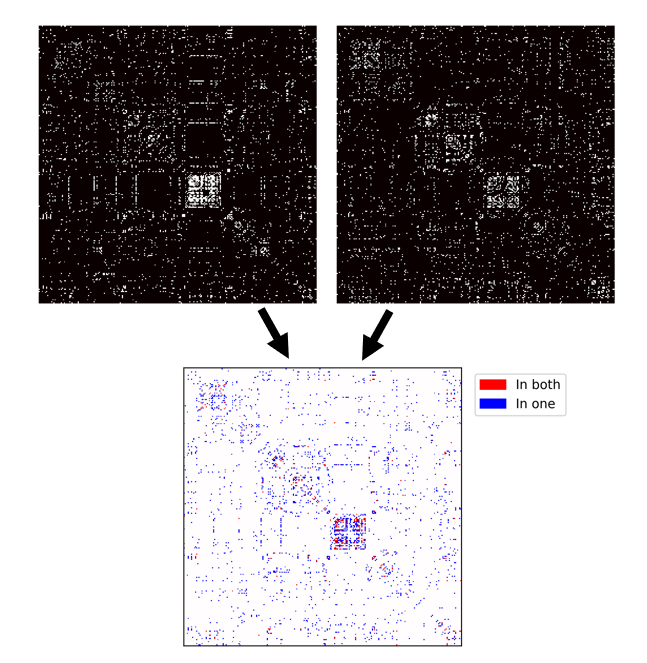
\includegraphics[height=3in]{ch4-network-intersection-methods}
    \caption[Method for comparing connectivity arrays.]{The network similarity measure provides a way of comparing connectivity arrays without reference to a pre-defined network parcellations.}
	\label{fig:ch4-network-intersection-methods}
\end{figure}


\section{Results}


\subsection{Behavioral results}

Attention and comprehension measures were not related to modality of stimulus presentation (see Fig. \ref{fig:ch4-task-performance}). There was a trend towards difference in median FDRMS between scan modalities (paired t-test, $t = 1.94$, $p = 0.059$), so we also replicated analyses with a stricter motion threshold (no more than 10 percent outliers in a scan run). The main results from analysis of this 35 subject (116 scan runs) cohort were broadly consistent.

\begin{figure}[t]
	\centering
	\includegraphics[height=3in]{ch4-task-performance}
    \caption[Behavioral metrics of passage performance were unrelated to modality.]{Both the in-scanner comprehension question and out-of-scanner recall questionnaire were unrelated to the modality of presentation.}
	\label{fig:ch4-task-performance}
\end{figure}


\subsection{Activation results}

Differences related to modality fell into three categories: sensory processing areas, including the insula, superior temporal gyrus, and secondary visual processing areas; and hetero-modal association areas, most notably the inferior frontal gyrus and angular gyrus; and somato-motor regions, including the premotor cortex and lateral geniculate nucleus of the thalamus (Fig. \ref{fig:ch3-modality-differences-attn}). Areas showing greater activation in listening were focused on primary auditory cortex and the dorsal attention network.

In the case of comprehension, we found that there was lower path length within modules during rest, while there were decreases in between-network connectivity during language.

For the modality contrast, One of the main takeaways is that there is greater access between auditory and other areas during reading -- this runs counter to our hypothesis that there would be less access to these areas. Visual areas, on the other hand, show less internal connectivity, reflecting the de-clustering of these areas during reading. 

\subsection{Connectivity analyses}
There was a high degree of similarity between the areas that were activated in reading and in listening, reflecting the common language core. Fig. \ref{fig:ch3-reading-connectome-activations} shows the activation statistics for each node, relative to rest, plotted against each other. There was a very high correlation coefficient ($r = 0.00$), reflecting the high degree of shared activity patterns between listening and reading.


\section{Discussion}

% Fronto-parietal description
% Task-based neuroimaging provides us with a rich description of the functions of frontoparietal network. The frontoparietal network is an assembly of brain regions encompassing the lateral frontal and parietal cortices along with insular, anterior/mid cingulate, and inferior temporal areas that have been broadly implicated in a variety of higher-level cognitive tasks \citep{Fedorenko2013}. Some have described the frontoparietal network as supporting active and adaptive online control, initiating and adjusting goal-directed mental systems \citep{Dosenbach2007}, while others have proposed a more general superordinate role in directing cognition \citep{Niendam2012}. The most obvious relationship of the frontoparietal network to language is its proximity to Broca’s area, known for its critical role in language articulation. Rather than thinking of this area (traditionally, Brodmann areas 44 and 45) as exclusively or primarily language-related, it has been argued that Broca’s area supports hierarchical executive processing, such as the segmentation (``chunking'') of auditory language and the flexible combination of words \citep{Koechlin2006}. Thus, while Broca's area plays a role in the unification of representations, prefrontal cortex (and the larger frontoparietal network) may play a higher-level control and initiating role in language and other processes \citep{Hagoort2005}. 

% Right hemisphere
% Our findings show that in stronger readers, the left frontoparietal RSN is expanded to include portions of the right posterior middle and superior temporal cortex.  These regions may play a number of roles in more skilled readers.  First, these right hemisphere regions are homologues of important left hemisphere language areas. The left posterior superior and middle temporal gyri are major secondary processing areas for written and auditory word stimuli \citep{Price2012}. In the right hemisphere, these areas are understood to play a complementary role, with a sensitivity to both emotional and prosodic elements \citep{Jung-Beeman2005}. Thus, the expansion of the frontoparietal network to these homologues could represent greater ``recruitment'' of complimentary language areas, facilitating  the integration of language-related information.  Secondly, these right hemisphere areas are subregions of the generally bilateral ventral attention RSN \citep{Yeo2011}.  Nonetheless in task-based studies, this network shows more of a right-sided bias \citep{Fox2006}.  As such, good readers may be better at integrating visual information with more high-order information.  These explanations need not be mutually exclusive.

% Ventral attention network
% While we found an expansion of the left frontoparietal RSN to regions of the ventral attention RSN in good readers, we did not find an association between variation in the ventral attention RSN itself and individual differences in reading ability. The ventral attention network detects salient or unexpected stimuli in the environment \citep{Vossel2014}. In this way the ventral attention network can act as a ‘circuit breaker’ for the dorsal system to help reorient attention \citep{Corbetta2002}. It may thus help orient individuals to new information from the visual environment (i.e. text) and, by coupling stimulus-driven attentional areas with the frontoparietal network, it may help construct updated mental representations of linguistic material. The leftward aspects of the ventral attention network underlie crucial reading-related areas, including occipito-temporal cortex, which performs orthographic processing, and temporo-parietal cortex, important for semantic binding \citep{Taylor2013}. The absence of reading-related variance associated with the entire bilateral RSN may reflect the diversity of functions that these areas serve in basic visual and auditory processing, as well as language and reading. 






\begin{figure}[t]
	\centering
	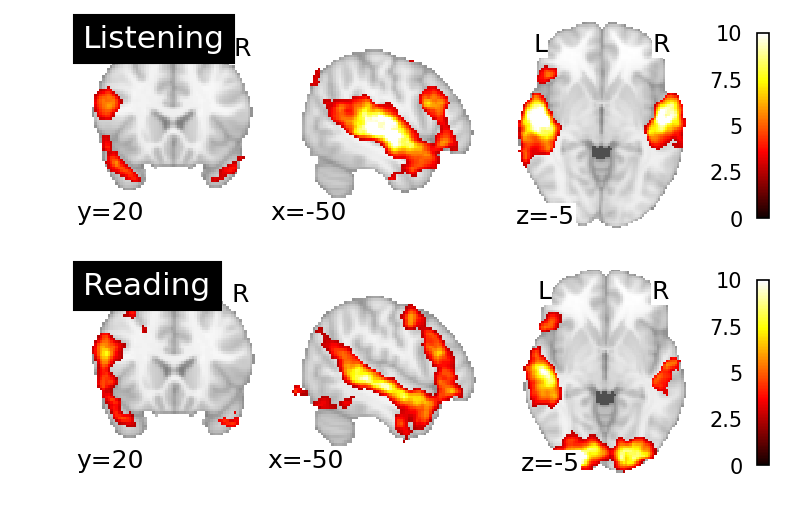
\includegraphics[height=3in]{ch4-modality-comparison-rest}
    \caption[Large overlap between listening and reading activation.]{Both the in-scanner comprehension question and out-of-scanner recall questionnaire were unrelated to the modality of presentation.}
	\label{fig:ch4-modality-comparison-rest}
\end{figure}


\begin{figure}[t]
	\centering
	\includegraphics[height=3in]{ch4-modality-comparison-rest-connectome}
    \caption[Large overlap between listening and reading activation in the connectome space.]{When projected into the node space, there was very strong correlation between activity in one and the other.}
	\label{fig:ch4-modality-comparison-rest-connectome}
\end{figure}


\begin{figure}[t]
	\centering
	\includegraphics[height=3in]{ch4-similarity-matrix-all}
    \caption[Auditory network organization is more similar for all subjects than it is for reading.]{}
	\label{fig:ch4-modality-network-similarity}
\end{figure}

\begin{figure}[t]
	\centering
	\includegraphics[height=3in]{ch4-similarity-matrix-reading}
    \caption[Network similarity between listening and reading predicts word efficiency.]{When projected into the node space, there was very strong correlation between activity in one and the other.}
	\label{fig:ch4-modality-network-similarity}
\end{figure}


\begin{figure}[t]
	\centering
	\includegraphics[height=3in]{ch4-similarity-matrix-reading}
    \caption[Diversity of between-network connections predominates on .... ]{Subjects that have more modular architectures are able to do it through greater hub... }
	\label{fig:ch4-modality-network-similarity}
\end{figure}

% Look at nodes that show increased participation coefficient across each different task. 
